\begin{figure*}[t]
\centering
\subfloat[Human Audit\label{tab:human_validation}]{\parbox[t][2.9cm][t]{0.24\textwidth}{\centering\vspace*{0.3cm}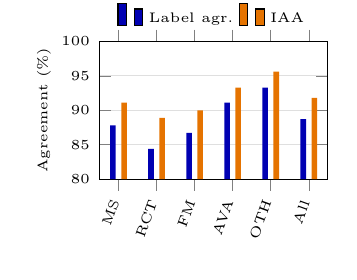
\begin{tikzpicture}\begin{axis}[ymajorgrids, grid style={gray!25}, tick label style={font=\tiny}, label style={font=\tiny}, title style={font=\tiny}, legend style={font=\tiny, draw=none, fill=none, at={(0.5,1.02)}, anchor=south}, legend columns=3, scale only axis, width=2.9cm, height=1.75cm, legend style={overlay}, ylabel shift=-3pt, ybar, bar width=2pt, symbolic x coords={MS,RCT,FM,AVA,OTH,All}, xtick={MS,RCT,FM,AVA,OTH,All}, x tick label style={rotate=70,anchor=east}, ylabel={Agreement (\%)}, ymin=80, ymax=100, legend columns=2]\addplot[fill=blue!70!black,draw=none] coordinates {(MS,87.80)(RCT,84.40)(FM,86.70)(AVA,91.10)(OTH,93.30)(All,88.70)};\addplot[fill=orange!90!black,draw=none] coordinates {(MS,91.10)(RCT,88.90)(FM,90.00)(AVA,93.30)(OTH,95.60)(All,91.80)};\legend{Label agr.,IAA}\end{axis}\end{tikzpicture}}}\hfill
\subfloat[Linguistic Profile\label{tab:dataset_characteristics}]{\parbox[t][2.9cm][t]{0.24\textwidth}{\centering\vspace*{0.3cm}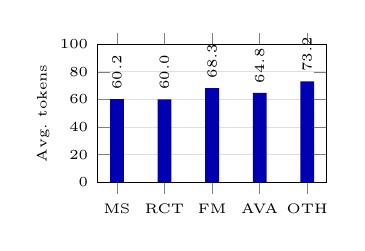
\begin{tikzpicture}\begin{axis}[ymajorgrids, grid style={gray!25}, tick label style={font=\tiny}, label style={font=\tiny}, title style={font=\tiny}, legend style={font=\tiny, draw=none, fill=none, at={(0.5,1.02)}, anchor=south}, legend columns=3, scale only axis, width=2.9cm, height=1.75cm, legend style={overlay}, ylabel shift=-3pt, ybar, bar width=5pt, symbolic x coords={MS,RCT,FM,AVA,OTH}, xtick={MS,RCT,FM,AVA,OTH}, ylabel={Avg.\ tokens}, ymin=0, ymax=100, nodes near coords={\pgfmathprintnumber[fixed,zerofill,precision=1]{\pgfplotspointmeta}}, nodes near coords style={font=\fontsize{3.5}{4}\selectfont, rotate=90, anchor=west}]\addplot[fill=blue!70!black,draw=none] coordinates {(MS,60.18)(RCT,60.04)(FM,68.34)(AVA,64.77)(OTH,73.23)};\end{axis}\end{tikzpicture}}}\hfill
\subfloat[Multi-Label Evaluation\label{tab:multilabel}]{\parbox[t][2.9cm][t]{0.24\textwidth}{\centering\vspace*{0.3cm}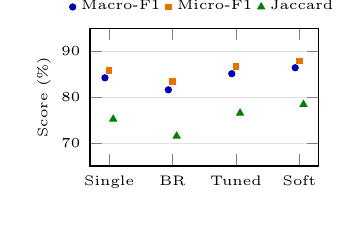
\begin{tikzpicture}\begin{axis}[ymajorgrids, grid style={gray!25}, tick label style={font=\tiny}, label style={font=\tiny}, title style={font=\tiny}, legend style={font=\tiny, draw=none, fill=none, at={(0.5,1.02)}, anchor=south}, legend columns=3, scale only axis, width=2.9cm, height=1.75cm, legend style={overlay}, ylabel shift=-3pt, symbolic x coords={Single,BR,Tuned,Soft}, xtick={Single,BR,Tuned,Soft}, ylabel={Score (\%)}, ymin=65, ymax=95]\addplot[only marks,mark=*,mark size=1.1pt,color=blue!70!black,xshift=-1.5pt] coordinates {(Single,84.20)(BR,81.60)(Tuned,85.10)(Soft,86.40)};\addplot[only marks,mark=square*,mark size=1.0pt,color=orange!90!black] coordinates {(Single,85.80)(BR,83.40)(Tuned,86.70)(Soft,87.90)};\addplot[only marks,mark=triangle*,mark size=1.4pt,color=green!50!black,xshift=1.5pt] coordinates {(Single,75.20)(BR,71.50)(Tuned,76.50)(Soft,78.40)};\legend{Macro-F1,Micro-F1,Jaccard}\end{axis}\end{tikzpicture}}}\hfill
\subfloat[Transfer to Real Posts\label{tab:domain_adaptation}]{\parbox[t][2.9cm][t]{0.24\textwidth}{\centering\vspace*{0.3cm}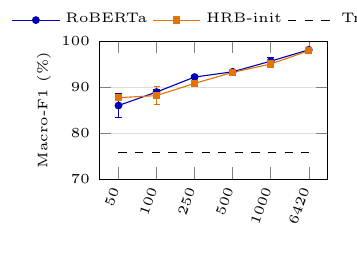
\begin{tikzpicture}\begin{axis}[ymajorgrids, grid style={gray!25}, tick label style={font=\tiny}, label style={font=\tiny}, title style={font=\tiny}, legend style={font=\tiny, draw=none, fill=none, at={(0.5,1.02)}, anchor=south}, legend columns=3, scale only axis, width=2.9cm, height=1.75cm, legend style={overlay}, ylabel shift=-3pt, symbolic x coords={50,100,250,500,1000,6420}, xtick={50,100,250,500,1000,6420}, x tick label style={rotate=70,anchor=east}, ylabel={Macro-F1 (\%)}, ymin=70, ymax=100]\addplot[mark=*,mark size=1.2pt,color=blue!70!black,error bars/.cd,y dir=both,y explicit,error bar style={line width=0.3pt}] coordinates {(50,86.03)+-(0,2.68)(100,88.97)+-(0,0.58)(250,92.23)+-(0,0.24)(500,93.37)+-(0,0.10)(1000,95.69)+-(0,0.79)(6420,98.16)+-(0,0.03)};\addplot[mark=square*,mark size=1.1pt,color=orange!90!black,error bars/.cd,y dir=both,y explicit,error bar style={line width=0.3pt}] coordinates {(50,87.74)+-(0,0.63)(100,88.19)+-(0,2.00)(250,90.85)+-(0,0.70)(500,93.24)+-(0,0.17)(1000,95.07)+-(0,0.56)(6420,97.97)+-(0,0.16)};\addplot[dashed,black,line width=0.4pt] coordinates {(50,75.87)(6420,75.87)};\legend{RoBERTa,HRB-init,Transfer}\end{axis}\end{tikzpicture}}}
\caption{Corpus profile, human audit, and transfer to real posts. (a)~Agreement of the majority human label with the intended label and inter-annotator agreement (IAA) on the stratified audit sample (90 posts per class). (b)~Average whitespace tokens per post (sentences: MS 3.8, RCT 3.5, FM 4.6, AVA 4.2, OTH 4.2; type--token ratio: MS 0.86, RCT 0.81, FM 0.85, AVA 0.86, OTH 0.83). (c)~Single-label, multi-label (binary relevance, BR; threshold-tuned), and soft-label evaluation on the audit sample (Hamming loss, \%: Single 5.7, BR 8.2, Tuned 6.5, Soft 5.9). (d)~Macro-F1 on CONSTRAINT@AAAI-2021 COVID-19 posts after fine-tuning on $k$ real posts (x-axis) from RoBERTa or from the \texttt{HealthRoleBench} classifier (HRB-init; mean $\pm$ standard deviation over seeds); the dashed line is HRB-init without real training data. \textcolor{red}{Values in (a) and (c) are placeholders from the earlier manuscript and will be replaced by the 450-post audit.}}
\label{fig:overview}
\vspace{-0.3cm}
\end{figure*}